%% uncomment to list all files in log
%\listfiles

\documentclass[12pt]{report}


\usepackage{fontspec}

%\setmainfont[Scale=MatchLowercase]{Lucida Bright}
%\setmonofont{FreeMono}
%\setmonofont{Source Code Pro}
\setmonofont[Scale=MatchLowercase]{Ubuntu Mono}

\usepackage[headings]{fullpage}

% national use characters 
%\usepackage{inputenc}

% ams mathematical symbols
\usepackage{amsmath,amssymb}

% added to support pandoc highlighting
\usepackage{microtype}

\usepackage{makeidx}

% add index and bibliographies to table of contents
\usepackage[nottoc]{tocbibind}

% postscript courier and times in place of cm fonts
%\usepackage{courier}
%\usepackage{times}

% extended coloring
\usepackage{color}
\usepackage[table,dvipsnames]{xcolor}
\usepackage{colortbl}

% advanced date formating
\usepackage{datetime}

%support pandoc code highlighting
\usepackage{fancyvrb}
\DefineShortVerb[commandchars=\\\{\}]{\|}
\DefineVerbatimEnvironment{Highlighting}{Verbatim}{commandchars=\\\{\}}
% Add ',fontsize=\small' for more characters per line

%tango style colors
% \usepackage{framed}
% \definecolor{shadecolor}{RGB}{255,255,255}
% \newenvironment{Shaded}{\begin{snugshade}}{\end{snugshade}}
% \newcommand{\KeywordTok}[1]{\textcolor[rgb]{0.13,0.29,0.53}{\textbf{{#1}}}}
% \newcommand{\DataTypeTok}[1]{\textcolor[rgb]{0.13,0.29,0.53}{{#1}}}
% \newcommand{\DecValTok}[1]{\textcolor[rgb]{0.00,0.00,0.81}{{#1}}}
% \newcommand{\BaseNTok}[1]{\textcolor[rgb]{0.00,0.00,0.81}{{#1}}}
% \newcommand{\FloatTok}[1]{\textcolor[rgb]{0.00,0.00,0.81}{{#1}}}
% \newcommand{\CharTok}[1]{\textcolor[rgb]{0.31,0.60,0.02}{{#1}}}
% \newcommand{\StringTok}[1]{\textcolor[rgb]{0.31,0.60,0.02}{{#1}}}
% \newcommand{\CommentTok}[1]{\textcolor[rgb]{0.56,0.35,0.01}{\textit{{#1}}}}
% \newcommand{\OtherTok}[1]{\textcolor[rgb]{0.56,0.35,0.01}{{#1}}}
% \newcommand{\AlertTok}[1]{\textcolor[rgb]{0.94,0.16,0.16}{{#1}}}
% \newcommand{\FunctionTok}[1]{\textcolor[rgb]{0.00,0.00,0.00}{{#1}}}
% \newcommand{\RegionMarkerTok}[1]{{#1}}
% \newcommand{\ErrorTok}[1]{\textbf{{#1}}}
% \newcommand{\NormalTok}[1]{{#1}}

%espresso style colors
% \usepackage{framed}
% \definecolor{shadecolor}{RGB}{42,33,28}
% \newenvironment{Shaded}{\begin{snugshade}}{\end{snugshade}}
% \newcommand{\KeywordTok}[1]{\textcolor[rgb]{0.26,0.66,0.93}{\textbf{{#1}}}}
% \newcommand{\DataTypeTok}[1]{\textcolor[rgb]{0.74,0.68,0.62}{\underline{{#1}}}}
% \newcommand{\DecValTok}[1]{\textcolor[rgb]{0.27,0.67,0.26}{{#1}}}
% \newcommand{\BaseNTok}[1]{\textcolor[rgb]{0.27,0.67,0.26}{{#1}}}
% \newcommand{\FloatTok}[1]{\textcolor[rgb]{0.27,0.67,0.26}{{#1}}}
% \newcommand{\CharTok}[1]{\textcolor[rgb]{0.02,0.61,0.04}{{#1}}}
% \newcommand{\StringTok}[1]{\textcolor[rgb]{0.02,0.61,0.04}{{#1}}}
% \newcommand{\CommentTok}[1]{\textcolor[rgb]{0.00,0.40,1.00}{\textit{{#1}}}}
% \newcommand{\OtherTok}[1]{\textcolor[rgb]{0.74,0.68,0.62}{{#1}}}
% \newcommand{\AlertTok}[1]{\textcolor[rgb]{1.00,1.00,0.00}{{#1}}}
% \newcommand{\FunctionTok}[1]{\textcolor[rgb]{1.00,0.58,0.35}{\textbf{{#1}}}}
% \newcommand{\RegionMarkerTok}[1]{\textcolor[rgb]{0.74,0.68,0.62}{{#1}}}
% \newcommand{\ErrorTok}[1]{\textcolor[rgb]{0.74,0.68,0.62}{\textbf{{#1}}}}
% \newcommand{\NormalTok}[1]{\textcolor[rgb]{0.74,0.68,0.62}{{#1}}}

%kete style colors
% \newenvironment{Shaded}{}{}
% \newcommand{\KeywordTok}[1]{\textbf{{#1}}}
% \newcommand{\DataTypeTok}[1]{\textcolor[rgb]{0.50,0.00,0.00}{{#1}}}
% \newcommand{\DecValTok}[1]{\textcolor[rgb]{0.00,0.00,1.00}{{#1}}}
% \newcommand{\BaseNTok}[1]{\textcolor[rgb]{0.00,0.00,1.00}{{#1}}}
% \newcommand{\FloatTok}[1]{\textcolor[rgb]{0.50,0.00,0.50}{{#1}}}
% \newcommand{\CharTok}[1]{\textcolor[rgb]{1.00,0.00,1.00}{{#1}}}
% \newcommand{\StringTok}[1]{\textcolor[rgb]{0.87,0.00,0.00}{{#1}}}
% \newcommand{\CommentTok}[1]{\textcolor[rgb]{0.50,0.50,0.50}{\textit{{#1}}}}
% \newcommand{\OtherTok}[1]{{#1}}
% \newcommand{\AlertTok}[1]{\textcolor[rgb]{0.00,1.00,0.00}{\textbf{{#1}}}}
% \newcommand{\FunctionTok}[1]{\textcolor[rgb]{0.00,0.00,0.50}{{#1}}}
% \newcommand{\RegionMarkerTok}[1]{{#1}}
% \newcommand{\ErrorTok}[1]{\textcolor[rgb]{1.00,0.00,0.00}{\textbf{{#1}}}}
% \newcommand{\NormalTok}[1]{{#1}}
%end pandoc code hacks

% jodliterate colors
\usepackage{color}
\definecolor{shadecolor}{RGB}{248,248,248}
% j control structures 
\definecolor{keywcolor}{rgb}{0.13,0.29,0.53}
% j explicit arguments x y m n u v
\definecolor{datacolor}{rgb}{0.13,0.29,0.53}
% j numbers - all types see j.xml
\definecolor{decvcolor}{rgb}{0.00,0.00,0.81}
\definecolor{basencolor}{rgb}{0.00,0.00,0.81}
\definecolor{floatcolor}{rgb}{0.00,0.00,0.81}
% j local assignments
\definecolor{charcolor}{rgb}{0.31,0.60,0.02}
\definecolor{stringcolor}{rgb}{0.31,0.60,0.02}
\definecolor{commentcolor}{rgb}{0.56,0.35,0.01}
% primitive adverbs and conjunctions
%\definecolor{othercolor}{rgb}{0.56,0.35,0.01}   
\definecolor{othercolor}{RGB}{0,0,255}
% global assignments
\definecolor{alertcolor}{rgb}{0.94,0.16,0.16}
% primitive J verbs and noun names
\definecolor{funccolor}{rgb}{0.00,0.00,0.00}    

\usepackage{framed}
\newenvironment{Shaded}{}{}
\newcommand{\KeywordTok}[1]{\textcolor{keywcolor}{\textbf{{#1}}}}
\newcommand{\DataTypeTok}[1]{\textcolor{datacolor}{{#1}}}
%\newcommand{\DecValTok}[1]{\textcolor{decvcolor}{{#1}}}
\newcommand{\DecValTok}[1]{{#1}} 
\newcommand{\BaseNTok}[1]{\textcolor{basencolor}{{#1}}}
\newcommand{\FloatTok}[1]{\textcolor{floatcolor}{{#1}}}
\newcommand{\CharTok}[1]{\textcolor{charcolor}{\textbf{{#1}}}}
\newcommand{\StringTok}[1]{\textcolor{stringcolor}{{#1}}}
\newcommand{\CommentTok}[1]{\textcolor{commentcolor}{\textit{{#1}}}}
\newcommand{\OtherTok}[1]{\textcolor{othercolor}{{#1}}} 
\newcommand{\AlertTok}[1]{\textcolor{alertcolor}{\textbf{{#1}}}}
%\newcommand{\FunctionTok}[1]{\textcolor{funccolor}{{#1}}}
\newcommand{\FunctionTok}[1]{{#1}}
\newcommand{\RegionMarkerTok}[1]{{#1}}
\newcommand{\ErrorTok}[1]{\textbf{{#1}}}
\newcommand{\NormalTok}[1]{{#1}}

% headers and footers
\usepackage{fancyhdr}
\pagestyle{fancy}

\fancyhead{}
\fancyfoot{}

%\fancyhead[LE,RO]{\slshape \rightmark}
%\fancyhead[LO,RE]{\slshape \leftmark}
\fancyfoot[C]{\thepage}
%\headrulewidth 0.4pt
%\footrulewidth 0 pt

%\addtolength{\headheight}{\baselineskip}

%\lfoot{\emph{Analyze the Data not the Drivel}}
%\rfoot{\emph{\today}}

% subfigure handles figures that contain subfigures
%\usepackage{color,graphicx,subfigure,sidecap}
\usepackage{graphicx,sidecap}
\usepackage{subfigure}
\graphicspath{{./inclusions/}}

% floatflt provides for text wrapping around small figures and tables
\usepackage{floatflt}

% tweak caption formats 
\usepackage{caption} 
\usepackage{sidecap}
%\usepackage{subcaption} % not compatible with subfigure

\usepackage{rotating} % flip tables sideways

% complex footnotes
%\usepackage{bigfoot}

% weird logos \XeLaTeX
\usepackage{metalogo}

% source code listings
\usepackage{listings}

% long tables
% \usepackage{longtable}

\newcommand{\HRule}{\rule{\linewidth}{0.5mm}}

% map LaTeX cross references into PDF cross references
\usepackage[
            %dvips,
            colorlinks,
            linkcolor=blue,
            citecolor=blue,
            urlcolor=blue,   % magenta, cyan default        
            pdfauthor={John D. Baker},
            pdftitle={Analyze the Data not the Drivel},
            pdfsubject={Blog},
            pdfcreator={MikTeX+LaTeXe with hyperref package},
            pdfkeywords={blog,wordpress},
            ]{hyperref}
           
% custom colors
\definecolor{CodeBackGround}{cmyk}{0.0,0.0,0,0.05}    % light gray
\definecolor{CodeComment}{rgb}{0,0.50,0.00}           % dark green {0,0.45,0.08}
\definecolor{TableStripes}{gray}{0.9}                 % odd/even background in tables

\lstdefinelanguage{bat}
{morekeywords={echo,title,pushd,popd,setlocal,endlocal,off,if,not,exist,set,goto,pause},
sensitive=True,
morecomment=[l]{rem}
}

\lstdefinelanguage{jdoc}
{
morekeywords={},
otherkeywords={assert.,break.,continue.,for.,do.,if.,else.,elseif.,return.,select.,end.
,while.,whilst.,throw.,catch.,catchd.,catcht.,try.,case.,fcase.},
sensitive=True,
morecomment=[l]{NB.},
morestring=[b]',
morestring=[d]',
}

% latex size ordering - can never remember it
% \tiny
% \scriptsize
% \footnotesize
% \small
% \normalsize
% \large
% \Large
% \LARGE
% \huge
% \Huge
 
% listings package settings  
\lstset{%
  language=jdoc,                                % j document settings
  basicstyle=\ttfamily\footnotesize,            
  keywordstyle=\bfseries\color{keywcolor}\footnotesize,
  identifierstyle=\color{black},
  commentstyle=\slshape\color{CodeComment},     % colored slanted comments
  stringstyle=\color{red}\ttfamily,
  showstringspaces=false,                       
  %backgroundcolor=\color{CodeBackGround},       
  frame=single,                                
  framesep=1pt,                                 
  framerule=0.8pt,                             
  rulecolor=\color{CodeBackGround},   
  showspaces=false,
  %columns=fullflexible,
  %numbers=left,
  %numberstyle=\footnotesize,
  %numbersep=9pt,
  tabsize=2,
  showtabs=false,
  captionpos=b
  breaklines=true,                              
  breakindent=5pt                              
}

\lstdefinelanguage{JavaScript}{
  keywords={typeof, new, true, false, catch, function, return, null, catch, switch, var, if, in, while, do, else, case, break},
  ndkeywords={class, export, boolean, throw, implements, import, this},
  ndkeywordstyle=\color{darkgray}\bfseries,
  sensitive=false,
  comment=[l]{//},
  morecomment=[s]{/*}{*/},
  morestring=[b]',
  morestring=[b]"
}

% C# settings
\lstdefinestyle{sharpc}{
language=[Sharp]C,
basicstyle=\ttfamily\scriptsize, 
keywordstyle=\bfseries\color{keywcolor}\scriptsize,
framerule=0pt
}

% for source code listing longer than two use smaller font
\lstdefinestyle{smallersource}{
basicstyle=\ttfamily\scriptsize, 
keywordstyle=\bfseries\color{keywcolor}\scriptsize,
framerule=0pt
}

\lstdefinestyle{resetdefaults}{
language=jdoc,
basicstyle=\ttfamily\footnotesize,  
keywordstyle=\bfseries\color{keywcolor}\footnotesize,                                                               
framerule=0.8pt 
}

% APL UTF8 code points listed for lstlisting processing
\makeatletter
\lst@InputCatcodes
\def\lst@DefEC{%
 \lst@CCECUse \lst@ProcessLetter
  ^^80^^81^^82^^83^^84^^85^^86^^87^^88^^89^^8a^^8b^^8c^^8d^^8e^^8f%
  ^^90^^91^^92^^93^^94^^95^^96^^97^^98^^99^^9a^^9b^^9c^^9d^^9e^^9f%
  ^^a0^^a1^^a2^^a3^^a4^^a5^^a6^^a7^^a8^^a9^^aa^^ab^^ac^^ad^^ae^^af%
  ^^b0^^b1^^b2^^b3^^b4^^b5^^b6^^b7^^b8^^b9^^ba^^bb^^bc^^bd^^be^^bf%
  ^^c0^^c1^^c2^^c3^^c4^^c5^^c6^^c7^^c8^^c9^^ca^^cb^^cc^^cd^^ce^^cf%
  ^^d0^^d1^^d2^^d3^^d4^^d5^^d6^^d7^^d8^^d9^^da^^db^^dc^^dd^^de^^df%
  ^^e0^^e1^^e2^^e3^^e4^^e5^^e6^^e7^^e8^^e9^^ea^^eb^^ec^^ed^^ee^^ef%
  ^^f0^^f1^^f2^^f3^^f4^^f5^^f6^^f7^^f8^^f9^^fa^^fb^^fc^^fd^^fe^^ff%
  ^^^^20ac^^^^0153^^^^0152%
  ^^^^20a7^^^^2190^^^^2191^^^^2192^^^^2193^^^^2206^^^^2207^^^^220a%
  ^^^^2218^^^^2228^^^^2229^^^^222a^^^^2235^^^^223c^^^^2260^^^^2261%
  ^^^^2262^^^^2264^^^^2265^^^^2282^^^^2283^^^^2296^^^^22a2^^^^22a3%
  ^^^^22a4^^^^22a5^^^^22c4^^^^2308^^^^230a^^^^2336^^^^2337^^^^2339%
  ^^^^233b^^^^233d^^^^233f^^^^2340^^^^2342^^^^2347^^^^2348^^^^2349%
  ^^^^234b^^^^234e^^^^2350^^^^2352^^^^2355^^^^2357^^^^2359^^^^235d%
  ^^^^235e^^^^235f^^^^2361^^^^2362^^^^2363^^^^2364^^^^2365^^^^2368%
  ^^^^236a^^^^236b^^^^236c^^^^2371^^^^2372^^^^2373^^^^2374^^^^2375%
  ^^^^2377^^^^2378^^^^237a^^^^2395^^^^25af^^^^25ca^^^^25cb%  
  ^^00}
\lst@RestoreCatcodes
\makeatother

% custom lengths used within minipages
\newcommand{\minindent}{17pt}


\makeindex

\begin{document}

\subsection*{\href{http://bakerjd99.wordpress.com/2010/08/12/c-k-raju-genius-or-crank-part-1/}{C. K. Raju: Genius or Crank (Part 1)}}
\addcontentsline{toc}{subsection}{C. K. Raju: Genius or Crank (Part 1)}


\noindent\emph{Posted: 12 Aug 2010 19:21:14}
\vspace{6pt}


%{[}caption id=``'' align=``alignleft'' width=``149'' caption=``Euclid's  first  proposition''{]}
%\href{http://new.math.uiuc.edu/math402/public/euclidsgeometry/elements.html}{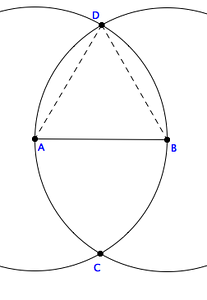
\includegraphics{969342389_3g8NU-M.png}}
\captionsetup[floatingfigure]{labelformat=empty}
\begin{floatingfigure}[r]{0.28\textwidth}
\centering
\href{http://new.math.uiuc.edu/math402/public/euclidsgeometry/elements.html}{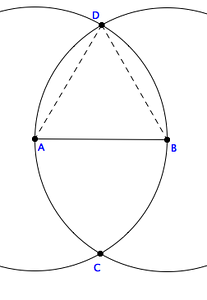
\includegraphics[width=0.24\textwidth]{969342389_3g8NU-M.png}}
\caption{Euclid's  first  proposition}
\label{fig:722X0}
\end{floatingfigure}Lately I have been amusing myself by working through
\href{http://www.amazon.com/Euclids-Elements-T-L-Heath-Translation/dp/1888009195/ref=pd\_sim\_b\_4}{Euclid's
Elements.} Despite studying mathematics in university, teaching it in
high school and \emph{occasionally} using it in my software-soaked day
job I never got around to reading Euclid.

Euclid is routinely lionized as the wellspring of axiomatic mathematics.
Before \emph{The Elements} mathematicians were \emph{clearly} out of
control! They were running around developing useful methods, (counting,
fractions, roots), and \emph{-- gasp -- making unjustified assertions!}

\emph{} Fortunately, \emph{The Elements} put an end to all that and
ushered in the endless age of rigorous axiomatic mathematics. I admire
mathematical rigor but my tiny brain can only take so much of it before
an all-pervading fog of befuddlement sets in. When I'm all fogged up
there are only a few options:

\begin{enumerate}
\item
  Reread and rework until the fog clears.
\item
  Press on and review later.
\item
  Give up and abase self.
\item
  Take a break.
\end{enumerate}
I'm a lazy
\href{http://www.urbandictionary.com/define.php?term=S.O.B.}{S.O.B.} so
option (4), take a break, comes up more often than it should. One of my
favorite ways to break away from mathematics is to read about it's
\emph{long} history. While tracing the history of \emph{The Elements} I
came across the writings of \href{http://ckraju.net/index.html}{C. K.
Raju.}

C. K. Raju has written a fascinating book: (the)
\href{http://books.google.com/books?id=jza\_cNJM6fAC\&pg=PA379\&lpg=PA379\&dq=C.+K.+Raju+Criticism\&source=bl\&ots=HEEAXlWhtW\&sig=7n3w6VnpLlYx2rQIMq7Lsa9uOcc\&hl=en\&ei=YY9hTNCvFMKBlAfdmcmLCw\&sa=X\&oi=book\_result\&ct=result\&resnum=5\&ved=0CCQQ6AEwBA\#v=onepage\&q\&f=false}{Cultural
Foundations of Mathematics: The Nature of Mathematical Proof and the
Transmission of the Calculus from India to Europe in the 16th c. CE.}
Raju's book is a bit hard to get your hands on. It's not on Amazon but
you can use \href{http://www.worldcat.org/}{World Cat} to find a copy
near you.

Raju's thesis consist of these major points:

\begin{enumerate}
\item
  Significant portions of the \emph{calculus} developed in India long
  before \href{http://en.wikipedia.org/wiki/Isaac\_Newton}{Newton} and
  \href{http://en.wikipedia.org/wiki/Gottfried\_Leibniz}{Leibniz} and
  Indian methods, particularly series expansions, came into Europe via
  16\textsuperscript{th} century Jesuit missionaries.
\item
  European notions of rigorous mathematical proof evolved from the needs
  of the Catholic Church to convert Muslims with
  \emph{impressive} iron-clad logical arguments. The old
  \href{http://writing2.richmond.edu/training/383/383restricted/bullshit.pdf}{baffle
  them with bullshit} tactic. Raju claims this \emph{theological}
  attitude worked it's way into mathematics and resulted in the
  \emph{bizarre western view} that deduction is superior to observation,
  experience and induction.
\item
  The ultimate source of eastern secular knowledge, (mostly Arab and
  Indian), was systematically suppressed and ``Hellenized'' by the
  Catholic Church. The church claimed all the ``good stuff'' in Arab
  texts originated with the ancient Greeks and had been \emph{merely
  preserved by Arab copycats.} It just wouldn't do to credit hated,
  (remember the crusades), enemies for their good ideas.
\item
  Insisting on rigorous proof when teaching mathematics, especially to
  children, is sterile and stupid.
\end{enumerate}
All of this reads like a mathematical
\href{http://www.danbrown.com/\#/home}{Dan Brown} novel and oddly the
Catholic Church is once again the villain. I was enjoying Raju's account
until this passage about
\href{http://en.wikipedia.org/wiki/Johannes\_Kepler}{Kepler}:

\begin{quotation}
\emph{Why, after all, was
\href{http://en.wikipedia.org/wiki/Tycho\_Brahe}{Tycho} so secretive
about his papers, not even allowing his trusted assistant Kepler to see
them? In any case, on Tycho's sudden death, Kepler obtained not just
Tycho's observations but also the rest of his papers which contained the
underlying theory. Being inclined towards heliocentrism, Kepler
transformed
\href{http://en.wikipedia.org/wiki/Nilakantha\_Somayaji}{Nilakantha's}
``Tychonic'' orbits to a heliocentric frame (a simple transformation).
This made Nilakantha's variable epicycles come out as ellipses. Being a
professional astrologer, Kepler was good at making up stories, and he
made up the story about how he had arrived at his results using Tycho's
data.}
\end{quotation}

In other words Kepler is a fraud and he ripped off one of the major
discoveries in astronomy, the elliptical orbits of planets, from Indian
astronomers. It's one thing to spin plausible stories about how parts of
calculus may have seeped into Europe from unacknowledged sources it's
another thing to posthumously accuse someone of fraud.

What would it take to make Raju's case? \emph{How about some hard
evidence!} What about Tycho's secret papers, do any of these documents
survive and do they contain references to Nilakantha? Now that would be
a smoking gun. Of course we don't know of any such papers \emph{but that
doesn't mean they didn't exist.} Proof by conspiracy is a very powerful
inference rule ---
\href{http://www.urbandictionary.com/define.php?term=troofer}{9/11
troofers} and \href{http://mw4.m-w.com/dictionary/ufologist}{ufologists}
swear by it! What about the claim that the transformation from
Nilakantha's variable epicycle \textbf{Earth centered system} to a
\textbf{Sun centered} elliptical orbit system is ``a simple
transformation.'' I rather doubt it's as simple as claimed and even if
the transformation was, to use the most abused word in mathematics ---
\emph{trivial}, it still misses the point. The major shift was to
abandon all pretense of \textbf{Earth centered systems} no matter how
mathematically sophisticated! Before Kepler astronomers and
mathematicians, in many cultures, toyed with the idea that planets orbit
the sun. After Kepler everyone had to grow up. Planets do orbit the sun
deal with it!

And it was precisely how Newton dealt with it that made calculus
something worth fighting over. Newton's unprecedented and monumental
proof that elliptical orbits are a mathematical consequence of the
inverse square law of gravity is the dividing line between modern and
early science. Nothing like it had ever been done before and even today
physics and mathematics students are given to chanting
\href{http://www.youtube.com/watch?v=-FucbvoFFy0}{we are not worthy}
when presented with this brilliant argument. Without Newton's use of the
calculus nobody but a few anal mathematicians would give a rat's ass
about who invented calculus.

In a later post I will argue that Raju discounts the importance of
independent and coequal mathematical discovery in his account.

%\captionsetup[floatingfigure]{labelformat=empty}
%\begin{figure}[htbp]
%\begin{floatingfigure}[l]{0.25\textwidth}
%\centering
%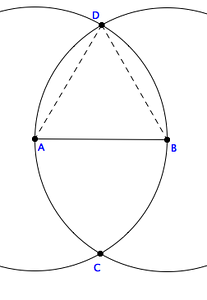
\includegraphics[width=0.23\textwidth]{969342389_3g8NU-M.png}
%\caption{~~~IMCAPTION~~~}
%\label{fig:722X0}
%\end{floatingfigure}
%\end{figure}



%\end{document}